\graphicspath{{main/chapter4/fig/}}

\chapter{AFF3CT Environment}

\section{Philosophy~\cite{Cassagne2019a}}

\subsection{High Performance}

\begin{itemize}
  \item performance -> langage C++
\end{itemize}

\subsection{Portability}

\subsection{Algorithmic Heterogeneity}

\subsection{Reproducible Science}

\section{Related Works}

\begin{itemize}
  \item \cmark~Bibliothèques FEC: \url{http://aff3ct.github.io/fec_libraries.html}
\end{itemize}

\begin{table}
  \centering
  \caption{\texttt{C}/\Cxx open source channel coding simulators/libraries.}
  \label{tab:fec_libraries_comparison}
  {\small\resizebox{\linewidth}{!}{
  \begin{tabular}{r | r | r | r | r | c | C{\simcolwidth}  C{\simcolwidth}  C{\simcolwidth}  C{\simcolwidth}  C{\simcolwidth}  C{\simcolwidth}  C{\simcolwidth}  C{\simcolwidth}  C{\simcolwidth}  C{\simcolwidth} }
  \multirow{4}{*}{\textbf{Name}}                                                                     &                  & \multirow{4}{*}{\textbf{Lines}} & \multicolumn{2}{c |}{\multirow{2}{*}{\textbf{Commit}}}           & \multirow{4}{*}{\textbf{License}} & \multirow{4}{*}{\rotatebox[origin=c]{70}{Polar}} & \multirow{4}{*}{\rotatebox[origin=c]{70}{LDPC}} & \multirow{4}{*}{\rotatebox[origin=c]{70}{Turbo}} & \multirow{4}{*}{\rotatebox[origin=c]{70}{Turbo P.}} & \multirow{4}{*}{\rotatebox[origin=c]{70}{BCH}} & \multirow{4}{*}{\rotatebox[origin=c]{70}{RS}} & \multirow{4}{*}{\rotatebox[origin=c]{70}{Conv.}} & \multirow{4}{*}{\rotatebox[origin=c]{70}{RA}} & \multirow{4}{*}{\rotatebox[origin=c]{70}{Rep.}} & \multirow{4}{*}{\rotatebox[origin=c]{70}{Erasure}} \\
                                                                                                     & \textbf{Contri-} &                                 & \multicolumn{2}{c |}{}                                           &                                   &        &        &        &        &        &        &        &        &        &         \\ \cline{4-5}
                                                                                                     & \textbf{butors}  &                                 & \multirow{2}{*}{\textbf{First}} & \multirow{2}{*}{\textbf{Last}} &                                   &        &        &        &        &        &        &        &        &        &         \\
                                                                                                     &                  &                                 &                                 &                                &                                   &        &        &        &        &        &        &        &        &        &         \\ \hline
                                                                                                                                                                                                                                                                 % Polar    LDPC     Turbo    TPC      BCH      RS       Conv.    RA       Rep.     Erasure
  \href{https://github.com/aff3ct/aff3ct                   }{AFF3CT}~\cite{Cassagne2019a}            &               11 &                             76k & 2016                            & 2019                           & MIT                               & \cmark & \cmark & \cmark & \cmark & \cmark & \cmark & \cmark & \cmark & \cmark & \xmark  \\
  \href{https://github.com/aicodix/code                    }{aicodix GmbH}~\cite{Aicodix}            &                1 &                              7k & 2018                            & 2020                           & Copyright                         & \xmark & \cmark & \xmark & \xmark & \cmark & \cmark & \xmark & \xmark & \xmark & \xmark  \\
  \href{http://www.eccpage.com                             }{eccpage}~\cite{ECCpage}                 &               20 &                               - & 1989                            & 2006                           & -                                 & \xmark & \cmark & \cmark & \xmark & \cmark & \cmark & \cmark & \xmark & \xmark & \cmark  \\
  \href{https://github.com/pjkundert/ezpwd-reed-solomon    }{EZPWD}~\cite{EZPWDRS}                   &                2 &                              6k & 2014                            & 2018                           & GPLv3                             & \xmark & \xmark & \xmark & \xmark & \xmark & \cmark & \xmark & \xmark & \xmark & \xmark  \\
  \href{https://github.com/Bulat-Ziganshin/FastECC         }{FastECC}~\cite{FastECC}                 &                2 &                              1k & 2015                            & 2018                           & Apache 2.0                        & \xmark & \xmark & \xmark & \xmark & \xmark & \cmark & \xmark & \xmark & \xmark & \xmark  \\
  \href{https://github.com/catid/fecal                     }{FEC-AL}~\cite{FEC-AL}                   &                1 &                              3k & 2018                            & 2018                           & BSD 3-Clause                      & \xmark & \xmark & \xmark & \xmark & \xmark & \xmark & \cmark & \xmark & \xmark & \cmark  \\
  \href{https://github.com/randombit/fecpp                 }{FECpp}~\cite{FECpp}                     &                1 &                              2k & 2009                            & 2018                           & -                                 & \xmark & \xmark & \xmark & \xmark & \xmark & \xmark & \xmark & \xmark & \xmark & \cmark  \\
  \href{https://github.com/gnuradio/gnuradio               }{GNURadio}~\cite{GNURadio}               &              192 &                            270k & 2006                            & 2019                           & GPLv3                             & \cmark & \cmark & \xmark & \xmark & \xmark & \xmark & \cmark & \xmark & \cmark & \xmark  \\
  \href{https://github.com/xdsopl/LDPC                     }{Inan}~\cite{Inan-LDPC}                  &                2 &                             13k & 2018                            & 2019                           & Copyright                         & \xmark & \cmark & \xmark & \xmark & \xmark & \xmark & \xmark & \xmark & \xmark & \xmark  \\
  \href{http://itpp.sourceforge.net                        }{IT++}~\cite{ITpp}                       &               20 &                            109k & 2005                            & 2018                           & GPLv3                             & \xmark & \cmark & \cmark & \xmark & \cmark & \cmark & \cmark & \xmark & \xmark & \xmark  \\
  \href{https://github.com/blegal/Fast_LDPC_decoder_for_x86}{Le Gal}~\cite{LeGal-LDPC}               &                1 &                             83k & 2015                            & 2019                           & -                                 & \xmark & \cmark & \xmark & \xmark & \xmark & \xmark & \xmark & \xmark & \xmark & \xmark  \\
  \href{https://github.com/catid/leopard                   }{Leopard}~\cite{Leopard}                 &                4 &                              5k & 2017                            & 2018                           & BSD 3-Clause                      & \xmark & \xmark & \xmark & \xmark & \xmark & \cmark & \xmark & \xmark & \xmark & \xmark  \\
  \href{https://github.com/quiet/libcorrect                }{libcorrect}~\cite{Libcorrect}           &                6 &                              5k & 2016                            & 2018                           & BSD 3-Clause                      & \xmark & \xmark & \xmark & \xmark & \xmark & \cmark & \cmark & \xmark & \xmark & \xmark  \\
  \href{https://github.com/radfordneal/LDPC-codes          }{Neal}~\cite{Neal-LDPC}                  &                1 &                              5k & 2006                            & 2012                           & Copyright                         & \xmark & \cmark & \xmark & \xmark & \xmark & \xmark & \xmark & \xmark & \xmark & \xmark  \\
  \href{https://gitlab.eurecom.fr/oai/openairinterface5g   }{OpenAir}~\cite{OpenAir}                 &              148 &                            740k & 2013                            & 2019                           & OAI Public                        & \xmark & \xmark & \cmark & \xmark & \xmark & \xmark & \xmark & \xmark & \xmark & \xmark  \\
  \href{http://openfec.org                                 }{OpenFEC}~\cite{OpenFEC}                 &                8 &                             55k & 2009                            & 2014                           & CeCCIL-C                          & \xmark & \cmark & \xmark & \xmark & \xmark & \cmark & \xmark & \xmark & \xmark & \xmark  \\
  \href{https://github.com/ArashPartow/schifra             }{Schifra}~\cite{Schifra}                 &                1 &                              7k & 2010                            & 2018                           & GPLv3                             & \xmark & \xmark & \xmark & \xmark & \xmark & \cmark & \xmark & \xmark & \xmark & \xmark  \\
  \href{https://github.com/catid/siamese                   }{Siamese}~\cite{Siamese}                 &                1 &                             11k & 2018                            & 2018                           & BSD 3-Clause                      & \xmark & \xmark & \xmark & \xmark & \xmark & \xmark & \cmark & \xmark & \xmark & \cmark  \\
  \href{https://github.com/tavildar/Polar                  }{Tavildar (Polar)}~\cite{Tavildar-Polar} &                1 &                              2k & 2016                            & 2017                           & -                                 & \cmark & \xmark & \xmark & \xmark & \xmark & \xmark & \xmark & \xmark & \xmark & \xmark  \\
  \href{https://github.com/tavildar/LDPC                   }{Tavildar (LDPC)}~\cite{Tavildar-LDPC}   &                1 &                              1k & 2016                            & 2016                           & -                                 & \xmark & \cmark & \xmark & \xmark & \xmark & \xmark & \xmark & \xmark & \xmark & \xmark  \\
  \href{http://www.the-art-of-ecc.com                      }{the-art-of-ecc}~\cite{The-art-of-ecc}   &                1 &                               - & 2006                            & 2009                           & Copyright                         & \xmark & \cmark & \cmark & \cmark & \cmark & \cmark & \cmark & \xmark & \xmark & \xmark  \\
  \href{https://github.com/ttsou/turbofec                  }{TurboFEC}~\cite{TurboFEC}               &                2 &                              4k & 2015                            & 2018                           & GPLv3                             & \xmark & \xmark & \cmark & \xmark & \xmark & \xmark & \xmark & \xmark & \xmark & \xmark  \\
  \end{tabular}
  }}
\end{table}

In the digital communications community, many scientists implement their own
simulation chain to validate their works.
Table~\ref{tab:fec_libraries_comparison} presents, to the best of our knowledge,
a list of currently available \verb|C|/\Cxx open source channel coding
simulators/libraries. We choose to compare with projects compiled as binaries,
since they aim at high throughput and low latency, as \AFFECT. Many open source
projects in Python or in MATLAB exist as well, but these tools are usually
slower than compiled binaries, and rather aim at prototyping.

Table~\ref{tab:fec_libraries_comparison} shows that, generally, the
\verb|C|/\Cxx FEC libraries target a single family or a small subset of channel
codes. As a consequence, a large effort is spent to re-develop similar features,
since all those libraries and tools share many characteristics (except the
channel code itself). \AFFECT attempts to lower this redundancy by releasing a
full simulator/library that consistently supports a wide range of channel codes
to the community. \AFFECT also tries to homogenize usage (command line, \Cxx
interfaces, etc.) for all code families.
Table~\ref{tab:fec_libraries_comparison} does not aim at comparing channel code
implementation performances. Instead, on the \AFFECT website, an overview of
software channel decoders state-of-the-art is provided for turbo, LDPC and polar
codes\footnote{FEC Software Decoders Hall of Fame: \url{http://aff3ct.github.io/hof_turbo.html}}.

\section{Use Cases}

\subsection{Simulator~\cite{Cassagne2017,Cassagne2017a}}

\begin{itemize}
  \item documentation
  \item résultats de simulation, comparateur BER/FER (travaux de Mehdi)
  \item multi-noeuds
\end{itemize}

\begin{table}
  \centering
  \caption{Specifications of the target processors.}
  \label{tab:simu_cpus_specs}
  {\resizebox{\linewidth}{!}{
  \begin{tabular}{l  l | l | l | c | c | c | c | c}
  \multicolumn{2}{c |}{\multirow{2}{*}{\textbf{CPU}}} & \multicolumn{2}{c |}{\textbf{SIMD instr.}} & \multirow{2}{*}{\textbf{\# Proc.}} & \textbf{\# Cores}  & \textbf{Freq.} & \multirow{2}{*}{\textbf{SMT}} & \textbf{Turbo} \\ \cline{3-4}
          &                                           & \textbf{Name} & \textbf{Size}              &                                    & \textbf{per Proc.} & (GHz)          &                               & \textbf{Boost} \\
  \hline
  ARM\R   & ThunderX2\R CN9975                        & NEON          & 128-bit                    & 2                                  &  28                & 2.00           & 4                             & \xmark         \\
  Intel\R & Xeon Phi\TM 7230                          & AVX-512F      & 512-bit                    & 1                                  &  64                & 1.30           & 4                             & \cmark         \\
% AMD\R   & Ryzen\TM 7 2700X                          & AVX2          & 256-bit                    & 1                                  &  8                 & 3.70           & 2                             & \cmark         \\
  Intel\R & Xeon\TM E5-2680 v3                        & AVX2          & 256-bit                    & 2                                  &  12                & 2.50           & 1                             & \xmark         \\
  Intel\R & Xeon\TM Gold 6140                         & AVX-512BW     & 512-bit                    & 2                                  &  18                & 2.30           & 2                             & \cmark         \\
  Intel\R & Xeon\TM Gold 6142                         & AVX-512BW     & 512-bit                    & 2                                  &  16                & 2.60           & 1                             & \xmark         \\
  \end{tabular}
  }}
\end{table}

\begin{figure}
  \centering
  \subfloat[][Simulator speedups.]{\includegraphics[width=0.70\textwidth]{simu/speedup/speedup}\label{plot:simu_speedup}}
  % \quad
  \\
  \subfloat[][Simulator throughputs.]{\includegraphics[width=0.70\textwidth]{simu/throughput/throughput}\label{plot:simu_throughput}}
  \caption{\AFFECT simulation of a (2048,1723) Polar code, FA-SCL decoder
    $L=32$, BPSK modulation, AWGN channel, $E_b/N_0$ = 4.5~dB (BER = 4.34e-10,
    FER = 5.17e-08).}
  \label{plot:simu_speedup_throughput}
\end{figure}

Figure~\ref{plot:simu_speedup} depicts the speedups achieved on various modern
CPU architectures detailed in Table~\ref{tab:simu_cpus_specs}, while
Figure~\ref{plot:simu_throughput} exposes the corresponding simulation
information throughputs. In Figure~\ref{plot:simu_speedup}, the speedups on each
architecture are computed with respect to the single thread simulation time on
the same architecture. Each run assigns at most one \AFFECT thread to each
hardware thread, thus, since the architectures have different number of hardware
threads, the presented speedups do not all have the same number of measurement
points. In Figure~\ref{plot:simu_speedup_throughput}, an $N=2048$ and $K=1723$
Polar code (FA-SCL decoder, $L=32$, 32-bit GZip \verb|0x04C11DB7| CRC) is
simulated with a BPSK modulation and over an AWGN channel ($E_b/N_0 = 4.5$~dB,
last SNR point of the blue curve in Figure~\ref{fig:intro_bfer_polar}). The
frozen bits of the polar code have been generated with the Gaussian
Approximation method (GA)~\cite{Trifonov2012}. The communication chain is fully
vectorized with the \MIPP wrapper~\cite{Cassagne2018} and multi-threaded with
\Cxy{11} threads. The vectorization is applied at the tasks level (c.f.
Section~\ref{sec:soft_archi}) to take advantage of the algorithms intrinsic
level of parallelism, when the multi-threaded parallelism is used, to reduce the
simulation time by multiplicating the number of concurrent communication chains,
thanks to the independence property of Monte Carlo simulations. In order to
achieve highest possible throughputs, the receiver part of the simulator is
configured to work with 8-bit fixed-point representation for real numbers. It
has been shown that this representation does not degrade the decoding
performances of the FA-SCL decoder~\cite{Leonardon2019}. However \AFFECT
algorithms implementations can also be run on other representations like
64/32-bit floating-point and 16-bit fixed-point. For all the CPU targets, the
code has been compiled with the \Cxx GNU compiler version 8.2.0 on Linux, with
the following optimization flags: \verb|-O3 -funroll-loops -march=native|. Note
that \AFFECT also works on Windows and macOS at the same level of performance.
The simulation scales rather well on the tested architectures. The data remains
in the CPU caches because of the moderate frame size ($N = 2048$). Scaling on
the Xeon\TM Gold 6142 is not as good as the other targets, because the
\textit{Intel\R Turbo Boost} technology is enabled on this platform: the CPU
runs at higher frequencies when the number of active cores is low. \AFFECT
effectively leverages the simultaneous multi-threading (SMT) technology. This is
especially true for the ThunderX2\R CN9975 and Xeon\TM Gold 6140 targets. The
SMT technology helps to improve the usage of the available instruction-level
parallelism.

\begin{table}
  \centering
  \caption{\AFFECT multi-node speedups (single node: $2\times$Xeon\TM E5-2680 v3).}
  \label{tab:simu_speedup_mpi}
% {\footnotesize%\resizebox{\linewidth}{!}{
  \begin{tabular}{r | r | r | r}
  \textbf{Nodes} & \textbf{Cores} & \textbf{Info. T/P} & \textbf{Speedup} \\
                 &                & (Mb/s)             &           \\
  \hline
   1             &  24            &  1950              &  1.00     \\
   2             &  48            &  3901              &  1.95     \\
%  3             &  72            &  5826              &  2.99     \\
   4             &  96            &  7793              &  4.00     \\
%  5             & 120            &  9731              &  4.99     \\
%  6             & 144            & 11691              &  5.99     \\
%  7             & 168            & 13644              &  7.00     \\
   8             & 192            & 15829              &  8.12     \\
%  9             & 216            & 17755              &  9.10     \\
% 10             & 240            & 19582              & 10.04     \\
  16             & 384            & 31640              & 16.22     \\
  32             & 768            & 63075              & 32.34     \\
  \end{tabular}
% }%}
\end{table}

Table~\ref{tab:simu_speedup_mpi} shows the multi-node scaling with the OpenMPI
library (version 3.1.2). The information throughput (T/P) and the speedup are
almost linear with the number of nodes: This is expected because there are very
few communications between the various MPI processes. Note that the super-linear
scaling is due to the measurements imprecision.

\textbf{Those aforementioned results demonstrate the high throughput
capabilities of \AFFECT.} For instance, when using 32 MPI nodes on the given
(2048,1723) polar code, it takes about one minute to estimate the $E_b/N_0=4.5$
dB SNR point (BER = 4.34e-10, FER = 5.17e-08).

\subsection{Library~\cite{Cassagne2019a}}

\begin{itemize}
  \item pleins d'implem autre que les décodeurs
  \item outil graphique avec des boîtes, projet Romain
  \item wrapper MATLAB (travaux de Kun)
\end{itemize}

As a FEC library, \AFFECT can be used programmatically, for instance in
\emph{Software Defined Radio} (SDR) contexts or in simulations. \AFFECT blocks
can be used in external projects without restriction. Compute intensive blocks
are optimized and vectorized to run fast on a single core. The library is
thread-safe; however, it is not multi-threaded by itself, in contrast to the
simulator. Instead, it is the responsibility of the user to manage
multi-threading.

\subsubsection{Software Functionalities}

The \AFFECT software functionalities can be decomposed in three main parts: the
\textit{codecs}, the \textit{modems} and the \textit{channels}. The codecs are
the main part of the toolbox. There is a broad range of supported codes listed
in Table~\ref{tab:lib_codecs}.

\begin{table}
  \centering
  \caption{List of supported channel codes (codecs).}
  \label{tab:lib_codecs}
% {\footnotesize%\resizebox{\linewidth}{!}{
  \begin{tabular}{ c | c | c }
  \multirow{2}{*}{\textbf{Channel Code}}   & \multirow{2}{*}{\textbf{Standards}} & \multirow{2}{*}{\textbf{Decoders}}     \\
                                           &                                     &                                        \\
  \hline
  \hline
  \multirow{5}{*}{\textbf{LDPC}}           & 5G (data), WiFi,                    & Scheduling: Flooding and H./V. Layered \\
                                           & WiMAX, WRAN,                        & Sum-Product Algorithm (SPA)            \\
                                           & 10 Gigabit Eth.,                    & Min-Sum (NMS, OMS)                     \\
                                           & DVB-S2, CCSDS                       & Approximate Min-Star (AMS)             \\
                                           & etc.                                & Bit Flipping: GallagerA/B/E, PPBF, WBF \\
  \hline
  \multirow{4}{*}{\textbf{Polar}}          &                                     & Successive Cancellation (SC)           \\
                                           & 5G                                  & Successive Cancellation List (SCL)     \\
                                           & (control channel)                   & CRC Aided SCL (CA-SCL, Adaptive SCL)   \\
                                           &                                     & Soft Cancellation (SCAN)               \\
  \hline
  \multirow{1}{*}{\textbf{Turbo Parallel}} & LTE (3G, 4G),                       & Turbo BCJR                             \\
  (single and double                       & DVB-RCS,                            & Turbo BCJR + Early Termination (CRC)   \\
  binary)                                  & CCSDS, etc.                         & Post proc.: Flip aNd Check (FNC)       \\
  \hline
  \multirow{2}{*}{\textbf{Turbo Product}}  & \multirow{2}{*}{WiMAX (opt.)}       & \multirow{2}{*}{Turbo Chase-Pyndiah}   \\
                                           &                                     &                                        \\
  \hline
  \multirow{3}{*}{\textbf{BCH}}            & CD, DVD,                            &                                        \\
                                           & SSD, DVB-S2,                        & Berlekamp-Massey + Chien search        \\
                                           & Bitcoin, etc.                       &                                        \\
  \hline
  \multirow{3}{*}{\textbf{Reed-Solomon}}   & CD, DVD,                            &                                        \\
                                           & SSD, DVB-T,                         & Berlekamp-Massey + Chien search        \\
                                           & ADSL, etc.                          &                                        \\
  \hline
  \multirow{1}{*}{\textbf{Convolutional}}  &                                     & BCJR - Maximum A Posteriori (MAP)      \\
  (single and double                       & NASA                                & BCJR - Linear Approximation            \\
  binary)                                  &                                     & BCJR - Max Approximation               \\
  \end{tabular}
% }%}
\end{table}

The codecs naturally encompass the encoders and decoders, but they can also
include puncturing patterns to shorten frames length according to some
communication standards. Most of the codec algorithms come from the literature,
while the others have been designed under
\AFFECT~\cite{Tonnellier2016a,Tonnellier2016b,Tonnellier2017,Leonardon2019}.
In channel coding, the decoder is the most time-consuming process, compared to
the puncturing and the encoding processes. This is why a specific effort is put
on ensuring the high computing performance of the decoders. Most of the decoding
algorithms have thus been optimized to satisfy high throughput and low latency
constraints~\cite{LeGal2015a,Cassagne2015c,Cassagne2016a,Cassagne2016b}. Those
optimizations generally involve a vectorized implementation, a tailored data
quantization and the use of fixed-point arithmetic.

In typical communication chains, it is necessary to adapt the digital signal
to the physical support. This operation is performed by the modulator and
conversely by the demodulator. \AFFECT comes with a rich set of modems to this
purpose. Table~\ref{tab:lib_modems} lists all the supported modems.

\begin{table}
  \centering
  \caption{List of supported modulations/demodulations (modems).}
  \label{tab:lib_modems}
  %{\footnotesize%\resizebox{\linewidth}{!}{
  \begin{tabular}{ c | c | c }
  \multirow{2}{*}{\textbf{Modem}}        & \multirow{2}{*}{\textbf{Standard}} & \multirow{2}{*}{\textbf{Characteristics}} \\
                                         &                                    &                                           \\
  \hline
  \hline
  \multirow{3}{*}{\textbf{N-PSK}}        & IEEE 802.16 (WiMAX)                &                                           \\
                                         & UMTS (2G, 2G+)                     & Phase-Shift Keying                        \\
                                         & EDGE (8-PSK), ...                  &                                           \\
  \hline
  \multirow{3}{*}{\textbf{N-QAM}}        & IEEE 802.16 (WiMAX)                &                                           \\
                                         & UMTS (2G, 2G+)                     & Quadrature Amplitude Modulation           \\
                                         & 3G, 4G, 5G, ...                    &                                           \\
  \hline
  \multirow{3}{*}{\textbf{N-PAM}}        & IEEE 802.16 (WiMAX)                &                                           \\
                                         & UMTS (2G, 2G+)                     & Pulse Amplitude Modulation                \\
                                         & 3G, 4G, 5G, ...                    &                                           \\
  \hline
  \multirow{2}{*}{\textbf{CPM}}          & GMSK, Bluetooth                    & Continuous Phase Modulation               \\
                                         & IEEE 802.11 FHSS                   & Coded (convolutional-based) modulation    \\
  \hline
  \multirow{2}{*}{\textbf{OOK}}          & IrDA (Infrared)                    & On-Off Keying                             \\
                                         & ISM bands                          & Used in optical communication systems     \\
  \hline
  \multirow{2}{*}{\textbf{SCMA}}         & \multirow{2}{*}{Considered for 5G} & Sparse Code Multiple Access               \\
                                         &                                    & Multi-user modulation                     \\
  \hline
  \multirow{2}{*}{\textbf{User defined}} & \multirow{2}{*}{-}                 & Constellation and order can be            \\
                                         &                                    & defined from an external file             \\
  \end{tabular}
  %}%}
\end{table}

\AFFECT supports several coded modulation/demodulation schemes like the
Continuous Phase Modulation (CPM)~\cite{Aulin1981a,Aulin1981b} and the Sparse
Code Multiple Access (SCMA) modulation~\cite{Nikopour2013,Ghaffari2017,
Ghaffari2019} (many codebooks are supported~\cite{AlteraSCMA,Wu2015,Cheng2015,
Zhang2016,Klimentyev2016,Song2017,Klimentyev2017}). It allows to easily combine
and evaluate the channel codes with several types of modulations. In the case of
the CPM, analogical wave shapes are also simulated. The other modulation schemes
are at the digital level.

For simulation purposes, it is crucial to emulate the behavior of the physical
layer. This is the role of the channel. There are many possible configurations
depending on the physics phenomena to simulate.
Table~\ref{tab:lib_channels} reports all the supported channels.

\begin{table}
  \centering
  \caption{List of supported channels.}
  \label{tab:lib_channels}
  % {\footnotesize%\resizebox{\linewidth}{!}{
  \begin{tabular}{ c | c | c }
  \multirow{2}{*}{\textbf{Channel}}      & \multirow{2}{*}{\textbf{Multi-user}} & \multirow{2}{*}{\textbf{Characteristics}}      \\
                                         &                                      &                                                \\
  \hline
  \hline
  \multirow{2}{*}{\textbf{AWGN}}         & \multirow{2}{*}{Yes}                 & \multirow{2}{*}{Additive White Gaussian Noise} \\
                                         &                                      &                                                \\
  \hline
  \multirow{2}{*}{\textbf{BEC}}          & \multirow{2}{*}{No}                  & \multirow{2}{*}{Binary Erasure Channel}        \\
                                         &                                      &                                                \\
  \hline
  \multirow{2}{*}{\textbf{BSC}}          & \multirow{2}{*}{No}                  & \multirow{2}{*}{Binary Symmetric Channel}      \\
                                         &                                      &                                                \\
  \hline
  \multirow{2}{*}{\textbf{Rayleigh}}     & \multirow{2}{*}{Yes}                 & \multirow{2}{*}{Flat Rayleigh fading channel}  \\
                                         &                                      &                                                \\
  \hline
  \multirow{2}{*}{\textbf{User defined}} & \multirow{2}{*}{Not yet}             & User can import noise samples                  \\
                                         &                                      & from an external file                          \\
  \end{tabular}
  %}%}
\end{table}

The channels involve complex floating-point computations. It is frequent to use
exponential and trigonometric operations. Those types of operations cost a large
amount of CPU cycles to be computed. As for the decoders, the channels have been
carefully optimized based on branch instructions reduction and massive
vectorization.

All these features are available from the simulator and in the library. Many
additional functional functionalities available are skipped here for concision.

\subsubsection{Illustrative Example}

\begin{listing}
  \inputminted[frame=lines,linenos]{C++}{main/chapter4/src/library/modules_allocation.cpp}
  \caption{Modules allocation.}
  \label{lst:library_modules_allocation}
\end{listing}

In this section the communication chain proposed in
Figure~\ref{fig:soft_archi_com_chain_task_module} is implemented with the
\AFFECT library. The first step is to allocate the modules. In
Listing~\ref{lst:library_modules_allocation} we chose to allocate modules on
the stack, but it is also possible to do the same on the heap. $K$ is the number
of information bits, $N$ is the frame size and $E$ is the number of erroneous
frames to simulate. One can notice that there is a module for the encoder and
for the decoder, this differs from
Figure~\ref{fig:soft_archi_com_chain_task_module} where \textit{encode} and
\textit{decode} are tasks of the codec module. In fact the codec module exists
in \AFFECT and it is an aggregation of the encoder and decoder modules. For
simplicity, we chose not to use the codec module here. In this basic example, a
repetition code is selected, it simply repeats the information bits $N/K$ times.

\begin{listing}
  \inputminted[frame=lines,linenos]{C++}{main/chapter4/src/library/sockets_binding.cpp}
  \caption{Sockets binding.}
  \label{lst:library_sockets_binding}
\end{listing}

The next step is to bind the sockets of successive tasks together (see
Listing~\ref{lst:library_sockets_binding}): The \textit{source} module
output socket \verb|src::sck::generate::U_K| is connected to the
input socket \verb|enc::sck::encode::U_K| of the \textit{encoder}, and so
on, for all the sockets of the tasks.

\begin{listing}
  \inputminted[frame=lines,linenos]{C++}{main/chapter4/src/library/tasks_execution.cpp}
  \caption{Tasks execution.}
  \label{lst:library_tasks_execution}
\end{listing}

The simulation is then started and each task is executed. In
Listing~\ref{lst:library_tasks_execution}, the whole communication chain is
executed multiple times, until the $E$ frame error limit is achieved (typically
$E = 100$ erroneous frames).

To propose an easy to use interface, sockets and tasks can be selected through
the \verb|[]| operator, which takes a \Cxx strongly typed enumerate. This way it
is possible to specialize the code depending on whether it is a socket or a
task. Strongly typed enumerates are checked at compile time (contrary to
standard enumerates), making it impossible to use wrong values.

\subsection{Prototyping~\cite{Cassagne2017,Cassagne2017a}}

\begin{itemize}
  \item hardware in the loop (travaux d'Olivier)
\end{itemize}

\section{Software Architecture}
\label{sec:soft_archi}

\AFFECT is developed in \Cxx in an object-oriented programming style. It
provides the fundamental blocks involved in building communication chains
(sources, modems, codecs, channels, ...). Those blocks are organized as
\textit{modules} and \textit{tasks}.

\textbf{Module:} A set of related tasks sharing some characteristics. For
instance, the \textit{modem} module contains the \textit{modulate} and
\textit{demodulate} tasks.

\textbf{Task:} An elementary processing performed on some data. For instance,
\textit{decode} or \textit{modulate} are tasks. The tasks are characterized by
their \textit{sockets}. A socket of a task defines an entry point through which
the task will consume and/or produce data. There are three kinds of sockets:
\textit{input}, \textit{output} and \textit{input/output}, following a
philosophy close to \emph{ports} in component-based development approaches.

\begin{figure}
  \centering
  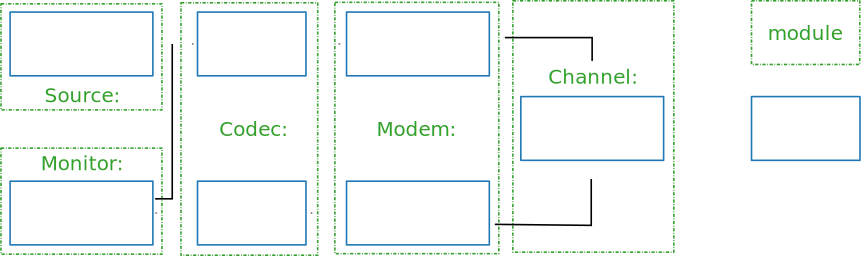
\includegraphics[width=1.00\linewidth]{soft_archi/com_chain_task_module}
  \caption{Modules and tasks.}
  \label{fig:soft_archi_com_chain_task_module}
\end{figure}

As a rule, a task is always a \emph{verb} and a module is always a \emph{noun}.
Modules are implemented as C++ classes, and tasks as class methods. \AFFECT
defines several abstract modules, for sources, codecs, modems, channels, etc. It
readily provides many implementations of those abstract classes; it is also
straightforward to add new ones.
Figure~\ref{fig:soft_archi_com_chain_task_module} presents common modules and
tasks typically found in a basic communication chain. It shows that the number
of tasks per module can vary depending on the module type.

\subsection{Factory}

\subsection{Module}

\subsection{Tools}

\subsection{Simulation}

\section{Sub-projects}

\subsection{\texttt{MIPP}}

\texttt{MIPP}: \url{https://github.com/aff3ct/MIPP}.

\subsection{\texttt{my\_project\_with\_aff3ct}}

\texttt{my\_project\_with\_aff3ct}: \url{https://github.com/aff3ct/my_project_with_aff3ct}.

\subsection{\texttt{polar\_decoder\_gen}}

\texttt{polar\_decoder\_gen}: \url{https://github.com/aff3ct/polar_decoder_gen}.

\subsection{\texttt{PyBER}}

\texttt{PyBER}: \url{https://github.com/aff3ct/PyBER}.

\subsection{\texttt{aff3ct.github.io}}

\texttt{aff3ct.github.io}: \url{https://github.com/aff3ct/aff3ct.github.io}.

\subsection{\texttt{cli}}

\texttt{cli}: \url{https://github.com/aff3ct/cli}.

\section{CI/CD}

\AFFECT's development leverages streamlined Continuous Integration (CI) process.
Each new commit to the version control repository triggers a comprehensive
sequence of tests to catch potential regressions. Regression tests are based on
past simulation results, validated from the state-of-the-art.

The CI process enables us to safely and confidently integrate contributed
features and improvements from the community to \AFFECT. It also helps to keep
the code review time by the core development team low-enough to swiftly
integrate such contributions into the master branch.

\subsection{Continuous Integration}
\begin{itemize}
  \item tests de compilation
  \item tests de régressions
\end{itemize}

\subsection{Continuous Delivery}

\section{Community and Impact}

\AFFECT is currently used in several industrial contexts for simulation purposes
(Turbo concept, Airbus, Thales, Huawei) and for specific developments (CNES,
Schlumberger, Airbus, Thales, Orange), as well as in academic projects (NAND
French National Agency project, IdEx CPU). The MIT license used in the project
is very permissive and gives confidence to industrial and academic partners, who
can then invest themselves and reuse parts of \AFFECT in their own projects
without any restrictions.

An important aspect of channel coding is the ability to reproduce
state-of-the-art results, because there are many possible configurations and it
is time-consuming to rediscover those configurations. This is why \AFFECT comes
with a large database of pre-simulated performance curves with all the required
parameters. Some research projects have been using \AFFECT as a
reference~\cite{Leonardon2018a,Leonardon2018b,Florian2018,Pignoly2018,
Ghanaatian2018,Poulenard2018,Cavatassi2019a,Cavatassi2019b,Cenova2019,
Guermouche2019,Krainyk2019,Wang2019,Wang2019a,Hsieh2020,Rush2020,Tasdighi2020}.
All pre-computed simulation results are available at a glance on the online
comparator\footnote{BER/FER comparator:
\url{http://aff3ct.github.io/comparator.html}}, with corresponding command lines
to reproduce them. Combined with the possibility to download \AFFECT last
builds\footnote{\AFFECT last builds:
\url{http://aff3ct.github.io/download.html}}, testing the reference
configurations, replicating the experiments and playing with parameters is
straightforward. \textbf{\AFFECT aims to achieve results easily reproducible by
the scientific community.}

It comes with a comprehensive documentation, to help using, modifying, extending
existing coding schemes, to potentially improve them or to adapt to other
domains. Moreover, \AFFECT can be used to prototype and evaluate hardware
implementations~\cite{Cassagne2017a}.

\subsection{Academics}
\subsection{Industrials}
\subsection{Contributors}

\section{Discussion}